%%%%%%%%%%%%%%%%%%%%%%%%%%%%%%%%%%%%%%%%%%%%%%%%%%%%%%%%%%%%%%%%%%%%%%%%%%%%%%%%
% Chapter 2: Conceptos
%%%%%%%%%%%%%%%%%%%%%%%%%%%%%%%%%%%%%%%%%%%%%%%%%%%%%%%%%%%%%%%%%%%%%%%%%%%%%%%%

%+++++++++++++++++++++++++++++++++++++++++++++++++++++++++++++++++++++++++++++++
% \section{Navegación robótica}
% \label{2:sec:4}
% https://en.wikipedia.org/wiki/Mobile_robot_navigation
La navegación robótica es la habilidad que permite a un robot móvil poder
localizarse en el entorno y poder moverse libremente por el mismo, a partir del
conocimiento extraído de las imágenes obtenidas del medio. El objetivo principal
es conocer por donde debe y no debe navegar con la idea de poder alcanzar un
punto de destino marcado previamente. 

En la robótica móvil es indispensable saber como moverse por el mundo, además de
conocer que situaciones de riesgo se han de evitar: colisiones, superficies
irregulares, zonas prohibidas, etc. 

Es posible subdividir la navegación dependiendo de la zona de estudio: de
interiores o de exteriores. En ambos casos las tecnologías pueden ser las
mismas, sin embargo mientras que en la localización en exteriores se suele hacer
uso de GPS, odometría mecánica, etc., en interiores es posible conseguir mejores
resultados con sensores ópticos como cámaras, odometría láser, etc.

La navegación robótica se caracteriza por estos tres tópicos:

\begin{itemize}
  \item \textbf{Localización:} localizarse en el entorno. 
  \item \textbf{Búsqueda de caminos:} búsqueda del camino más optimo para llegar
  a un objetivo. 
  \item \textbf{Mapeo robótico:} construcción de un mapa del entorno. 
\end{itemize}% nube de puntos

%+++++++++++++++++++++++++++++++++++++++++++++++++++++++++++++++++++++++++++++++
\subsection{Localización}
% http://www-math.mit.edu/~hajiagha/cars-fof.pdf
% http://ieeexplore.ieee.org/xpl/login.jsp?tp=&arnumber=1241767&url=http%3A%2F%2Fieeexplore.ieee.org%2Fxpls%2Fabs_all.jsp%3Farnumber%3D1241767

La localización es el primer tema a abordar en la navegación de un robot. El
objetivo es dar respuesta al '¿dónde estoy?', a través de conocer la posición
inicial, conocer la posición del punto de destino y autolocalizarse por el
entorno. La localización se puede dividir en dos grupos principales: basada en
puntos de referencias y basada en el análisis de las imágenes.

La localización basada en puntos de referencias se aprovecha en los puntos de
referencias que existen en el entorno y sobresalen de las imágenes de la escena
sin verse influenciados por otros factores de las escenas como los cambios en el
entorno o de los elementos que lo componen. Este tipo de puntos o marcas pueden
ser artificiales (líneas o flechas en un mapa o GPS) o naturales (puertas,
esquinas, senderos, etc.).

\begin{figure}[!th]
  \begin{center}
    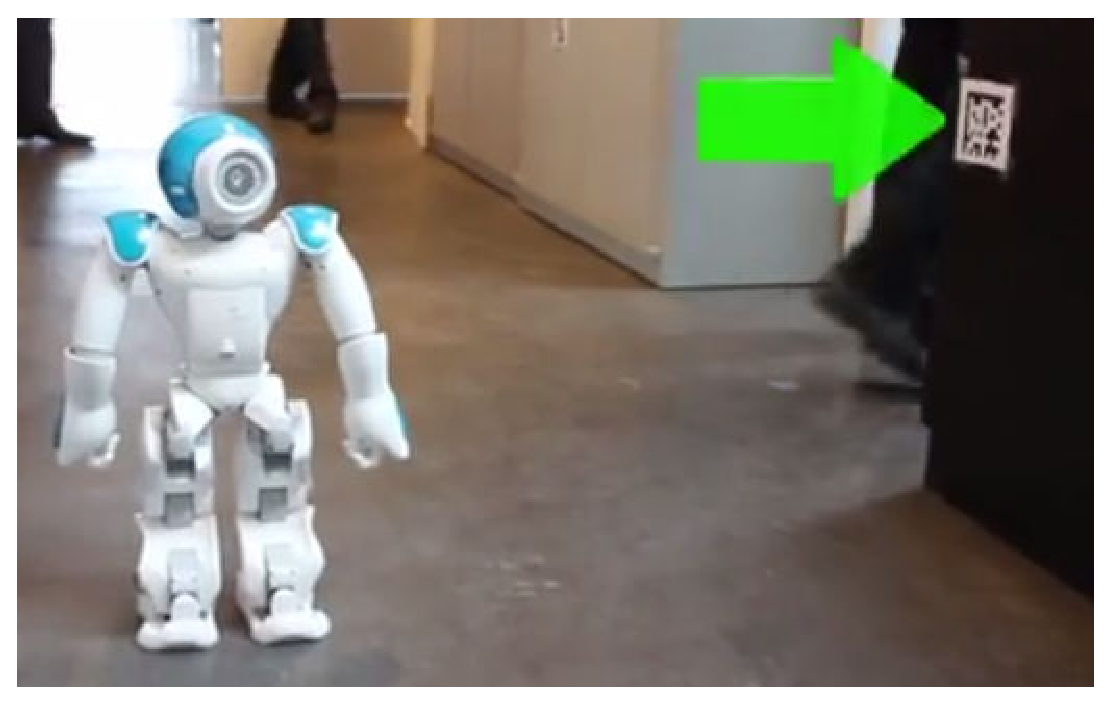
\includegraphics[width=0.5\textwidth]{images/cap2/LocalizacionMarcas.eps}
    \caption{Localización a través de código QR}
    \label{fig:LocalizacionMarcas}
  \end{center}
\end{figure}

Cuando este tipo de marcas no se pueden separar de las imágenes, porque bien no
se tienen puntos de referencia artificiales, o no se puede reconocer del propio
entorno marcas artificiales, se recurre a la localización basada en el análisis
de las imágenes capturadas. El primer paso es el 'auto-aprendizaje',
habitualmente navegar de forma autónoma y recoger las imágenes del entorno.
Estas imágenes se procesan, comparando los elementos en la escena de cada nueva
imagen recogida con la anterior y las imágenes que se tiene en el histórico,
obteniendo así la localización actual.

\begin{figure}[!th]
  \begin{center}
    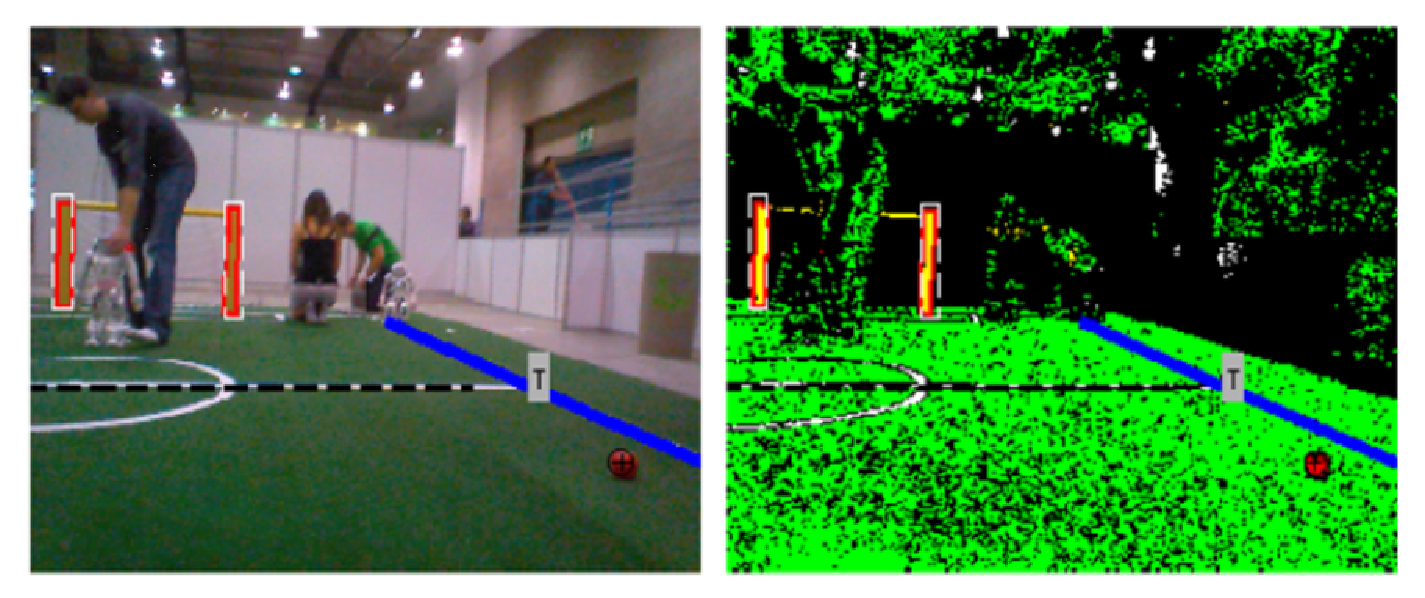
\includegraphics[width=0.7\textwidth]{images/cap2/LocalizacionImagenes.eps}
    \caption{Localización mediante los elementos de la escena}
    \label{fig:LocalizacionImagenes}
  \end{center}
\end{figure}

%--------------------------------------
\paragraph{Filtro de Kalman Extendido} \hspace{0pt} \\
% http://www.robolabo.etsit.upm.es/~inaki/coursework/kalman.pdf
% http://bibing.us.es/proyectos/abreproy/11879/fichero/PFC+Sergio+Pereira+Ruiz%252F7+-+Filtro+de+Kalman.pdf
% http://www.ual.es/personal/rgonzalez/documents/slam_ramon.pdf
El filtro de Kalman extendido (EKF) es un algoritmo que permite estimar la
posición de un robot a partir de la combinación de las ecuaciones de la
odometría y las medidas recogidas por los sensores. Se trata de un algoritmo muy
utilizado en sistemas de navegación.

El filtro de Kalman se basa en dos etapas: predicción y corrección.

En la etapa de predicción se tiene solamente en cuenta la odometría, cuyos datos
son almacenados en un vector de estado, los cuales se toman como una estimación
Este vector contiene las variables de interés, manteniendo el tiempo dos
posibles valores: el valor previsto (a priori) y el valor corregido (a
posteriori).

En la etapa de corrección, se introducen las medidas de los sensores. Con  la
odometría y los sensores, se calcula la diferencia entre el valor esperado y el
real, se obtiene la matriz de covarianza del sensor y se obtiene la Ganancia de
Kalman (determina cuanto se debe corregir la estimación). Finalmente se corrigen
los valores del vector de estado después de las nuevas observaciones.

Conforme pasa el tiempo crece la imprecisión, por lo que las etapas se repiten
sucesivamente con el fin de reducir la imprecisión.

\begin{figure}[!th]
  \begin{center}
    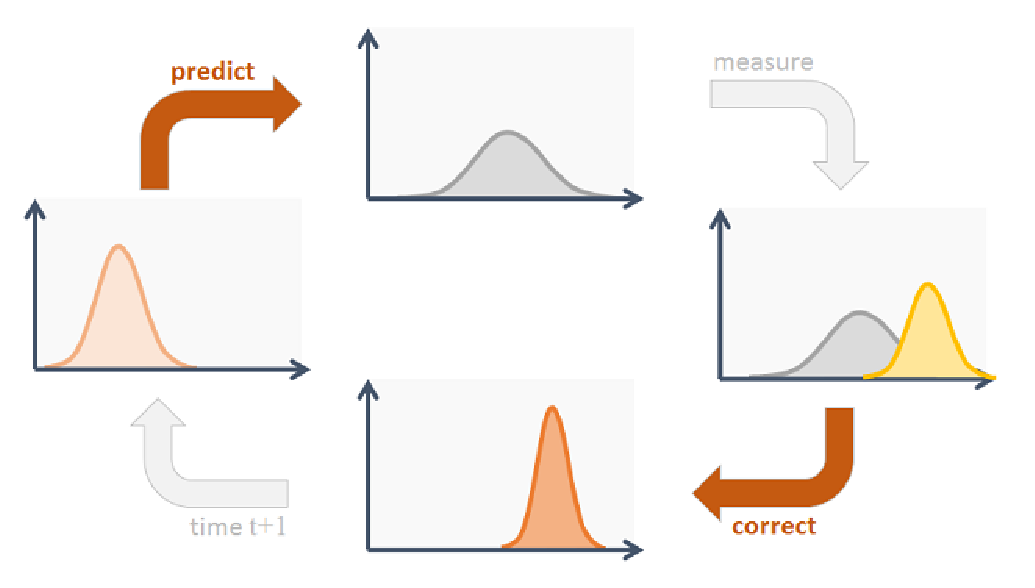
\includegraphics[width=0.7\textwidth]{images/cap2/Kalman.eps}
    \caption{Esquema del filtro de Kalman extendido}
    \label{fig:Kalman}
  \end{center}
\end{figure}

%+++++++++++++++++++++++++++++++++++++++++++++++++++++++++++++++++++++++++++++++
\subsection{Búsqueda de caminos}
% https://en.wikipedia.org/wiki/Motion_planning
% http://correll.cs.colorado.edu/?p=965111
% http://ais.informatik.uni-freiburg.de/teaching/ss11/robotics/slides/18-robot-motion-planning.pdf
% http://rabida.uhu.es/dspace/bitstream/handle/10272/5501/Nuevas_aportaciones_en_algoritmos_de_planificacion.pdf?sequence=2
La búsqueda de caminos permite hallar el conjunto de movimientos que permite a
un robot encontrar el camino más óptico hasta llegar a su objetivo, para no
solamente llegar en el menor tiempo posible, sino también evitar por el camino
los obstáculos que hagan peligrar el estado del robot o simplemente le retrasen.

El problema de la búsqueda de caminos ha sido ampliamente estudiado, existiendo
múltiples algoritmos para solventar este problema. 

Entre los métodos más conocidos están los 'roadmap', los cuales se basan en
construir una descripción de todo el espacio libre en el plano mediante un
grafo. Posteriormente los nodos del grafo se van conectando a partir de las
distancias más cortas entre sí, formando todos los caminos posibles, entre los
que se encuentra el más óptimo.

\begin{figure}[!th]
  \begin{center}
    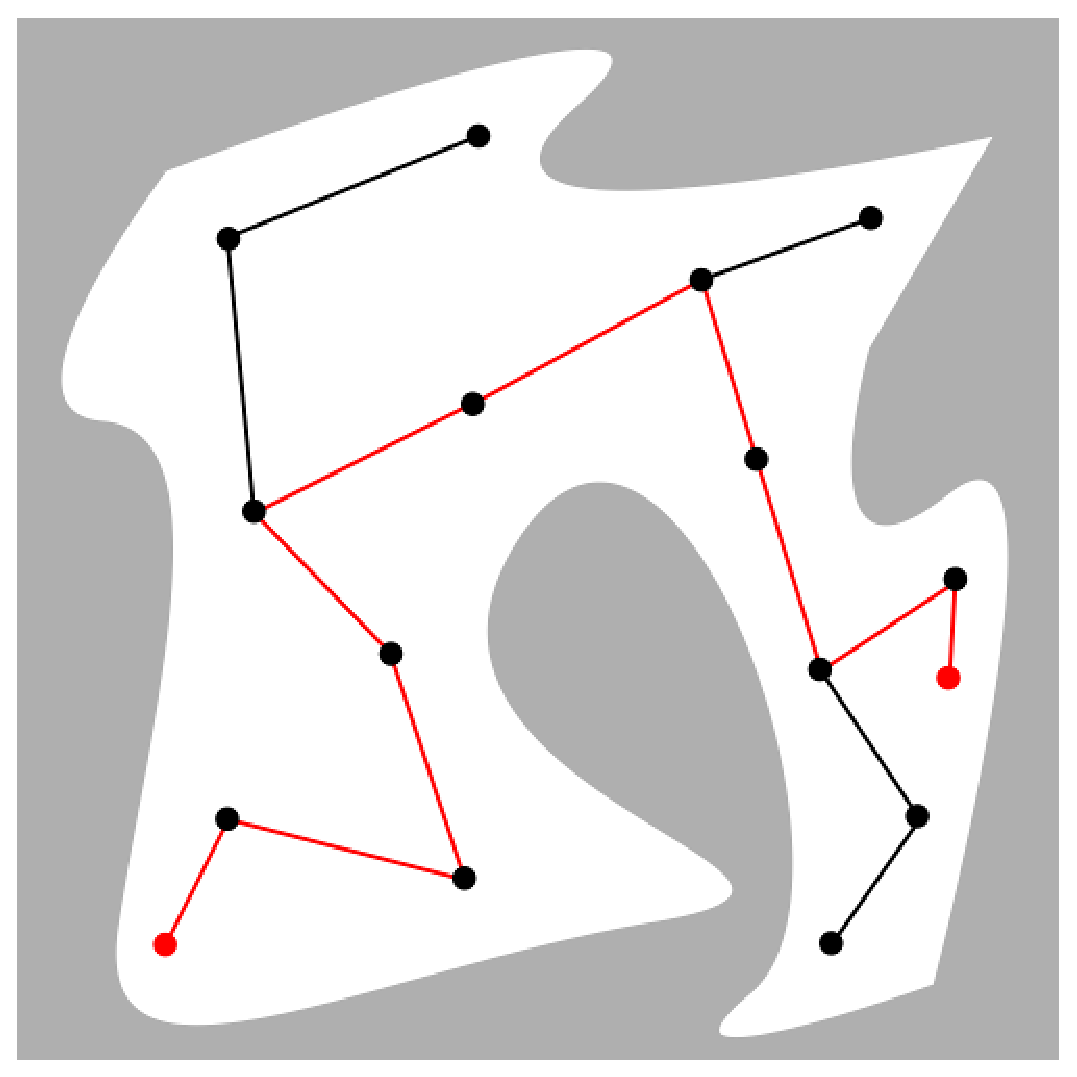
\includegraphics[width=0.5\textwidth]{images/cap2/BusquedaCaminosRoadmap.eps}
    \caption{Ejemplo de un 'roadmap'}
    \label{fig:BusquedaCaminosRoadmap}
  \end{center}
\end{figure}

Por otra parte, existen los métodos de descomposición en celdas, que en vez de
representar el entorno en un grafo, dividen el espacio libre de colisiones en un
conjunto de celdas. 

En los últimos años han surgido métodos alternativos que permiten dar solución a
la complejidad del entornos y las restricciones cinemáticas que puede presentar
un robot en la búsqueda de caminos, son los algoritmos de generación aleatoria,
el más famoso es el RRT o 'Rapidly Exploring Random Trees', muy utilizados en la
navegación autónoma. Este algoritmo se basa en la construcción al azar de un 
árbol que va creciendode manera incremental mediante la captura de nuevas
muestras del entorno.

%+++++++++++++++++++++++++++++++++++++++++++++++++++++++++++++++++++++++++++++++
\subsection{Mapeo robótico}
% https://en.wikipedia.org/wiki/Robotic_mapping
% https://en.wikipedia.org/wiki/3D_reconstruction_from_multiple_images
% Introduccion sobre el mapeo en robotica, que es porque...

La construcción de un mapa constituye el objetivo final de la navegación
robótica. Al igual que en la cartografía, un mapa representa toda la información
conocida acerca de un entorno: dimensiones del entorno, orografía, localización
de los obstáculos, etc. En robótica la utilización de un mapa es de gran
utilidad ya que permite tener un registro histórico de aquellas lugares que ya
ha visitado en el pasado, evitando así visitar zonas peligrosas o irrelevantes.

Los mapas se pueden representar de diferentes formas:

\begin{itemize}
  \item \textbf{Mapa métrico:} representación bidimensional del espacio y todos
  los objetos que lo rodean. Aunque la posición de los obstáculos es bastante
  aproximada a la realidad, deja de lado información importante del entorno. Una
  ampliacion de este tipo de mapas es mediante una representación tridimensional
  a través de la disposición de una nube de puntos, siendo posible apreciar
  datos  importantes del entorno: orografía del terreno, altura de los
  obstáculos, imágenes más detalladas del entorno, etc.
  \item \textbf{Mapa topológico:} grafo en el que los nodos corresponden a los
  lugares y sus arcos a la distancia entre ellos. Permite tener un abstracto
  claro y sencillo de la relación de los obstáculos entre ellos.
\end{itemize}

%--------------------------------------
\paragraph{SLAM} \hspace{0pt} \\
% http://www.ual.es/personal/rgonzalez/documents/slam_ramon.pdf
% https://es.wikipedia.org/wiki/SLAM_%28rob%C3%B3tica%29
% http://ais.informatik.uni-freiburg.de/teaching/ss12/robotics/slides/12-slam.pdf
A pesar de que la navegación de un robot se ha divido en tres etapas, donde la
primera es la localización y la última lo construcción de un mapa, realmente un
robot autónomo es capaz de construir un mapa del entorno comenzando desde una
posición desconocida en el mismo.

SLAM (Simultaneous Localization And Mapping) es una técnica que permite a un
robot construir un mapa de un entorno desconocido a la vez que es capaz de
localizarse en el mismo mediane sus sensores. 

Uno de los factores más importantes a tener en cuenta es la incertidumbre: no se
conoce ni la posición ni el entorno, y no solo eso, los sensores no son
perfectos y pueden arrojar resultados que no son acordes a la realidad,  por lo
que la clave está en seguir un modelo probabilístico. Esta imprecisión puede
corregirse con el paso del tiempo recorriendo continuadamente.

% algo mas tecnico
% loop closure

SLAM toma como base el teorema de Bayes para dar solución del problema, mediante
el uso de algritmos como el Filtro de Kalman Extendido o los Mapas de ocupación
de eldillas. Por otra parte, uno de los retos a los que se enfrenta SLAM es al
'loop closure' (cierre de bucle). Se trata del problema de reconocer aquel lugar
del mapa que ya ha sido visitado previamente. El éxito del SLAM depende poder
detectar esta situación

Los principales problemas con los que cuenta SLAM radican en la complejidad que
se tiene en los entornos dinámicos donde muchos objetos en el mapa se mueven
libremente. Por otra parte, es una técnica muy exigente que no se puede utilizar
en grandes entornos con muchos objetos, ya que el coste computacional crece al
cuadrado conforme a los objetos contenidos en el mapa.

A pesar de ello, los resultados obtenidos por SLAM son muy atractivos, ya que
sin conocer ni la posición ni el mapa, un robot autónomo puede moverse
libremente por el, obteniendo al mismo tiempo un mapa del entorno. Por otra
parte esta técnica es bastante robusta ante el ruido provocado por lo sensores.

%++++++++++++++++++++++++++++++++++++++++++++++++++++++++++++++++++++++++++++++
